\documentclass[11pt, a4paper]{article}
\usepackage[text={17cm, 24cm}, left=2cm, top=3cm]{geometry}
\usepackage[czech]{babel}
\usepackage[utf8]{inputenc}
\usepackage[IL2]{fontenc}
\usepackage{mathtools, amssymb, amsthm}
\usepackage[hidelinks]{hyperref}
\usepackage{times}
\usepackage{graphicx}

\begin{document}

    \begin{titlepage}
        \begin{center}
            
            \textsc{\Huge{Vysoké učení technické v Brně}}
            \\
            \textsc{\huge{Fakulta informačních technologií}}
                
            \vspace{\stretch{0.382}}
            
            \LARGE{Typografie~a~publikování\,--\,4.~projekt}
            \\
            \Huge{Množiny a matematická sazba v~{\LaTeX}u}
               
            \vspace{\stretch{0.618}}
        
        \end{center}    
        \Large{\today \hfill Dmitrii Ivanushkin}
    \end{titlepage}

\section*{Definice množiny}
    \theoremstyle{definition}
    \newtheorem{definition}{Definice}
    \begin{definition}
        Množina je konečný nebo nekonečný souhrn objektů, ve kterých pořadí nemá žádný význam a násobnost je obecně také ignorována (na rozdíl od seznamu nebo multimnožiny)~\cite{CantorGeorg1845-1918.Auteurdutexte1894BzBd}.
    \end{definition}
    
    \subsection*{Sazba definicí}
    Použil jsem tady příkazy {\fontfamily{qcr}\selectfont \string\theoremstyle} a {\fontfamily{qcr}\selectfont \string\newtheorem}. Informace, týkající se použití příkazu z balíčku {\fontfamily{qcr}\selectfont amsthm} můžete najít tady~\cite{talbot2013}

\section{Interpretace množin}
    Pro lepší porozumění můžeme představit množiny pomocí diagramů. Například, Eulerovy kruhy a Vennův diagram.
    \begin{quote}
        \dots [Oni] se již dlouho používají jako prostředek k vyjádření vztahů mezi množinami pomocí vizuálních metafor, jako je „nesouvislost“ a „zadržování“ \dots \cite{GILJOSEPHYOSSI2002PSoP}
    \end{quote} 
    \begin{center}
        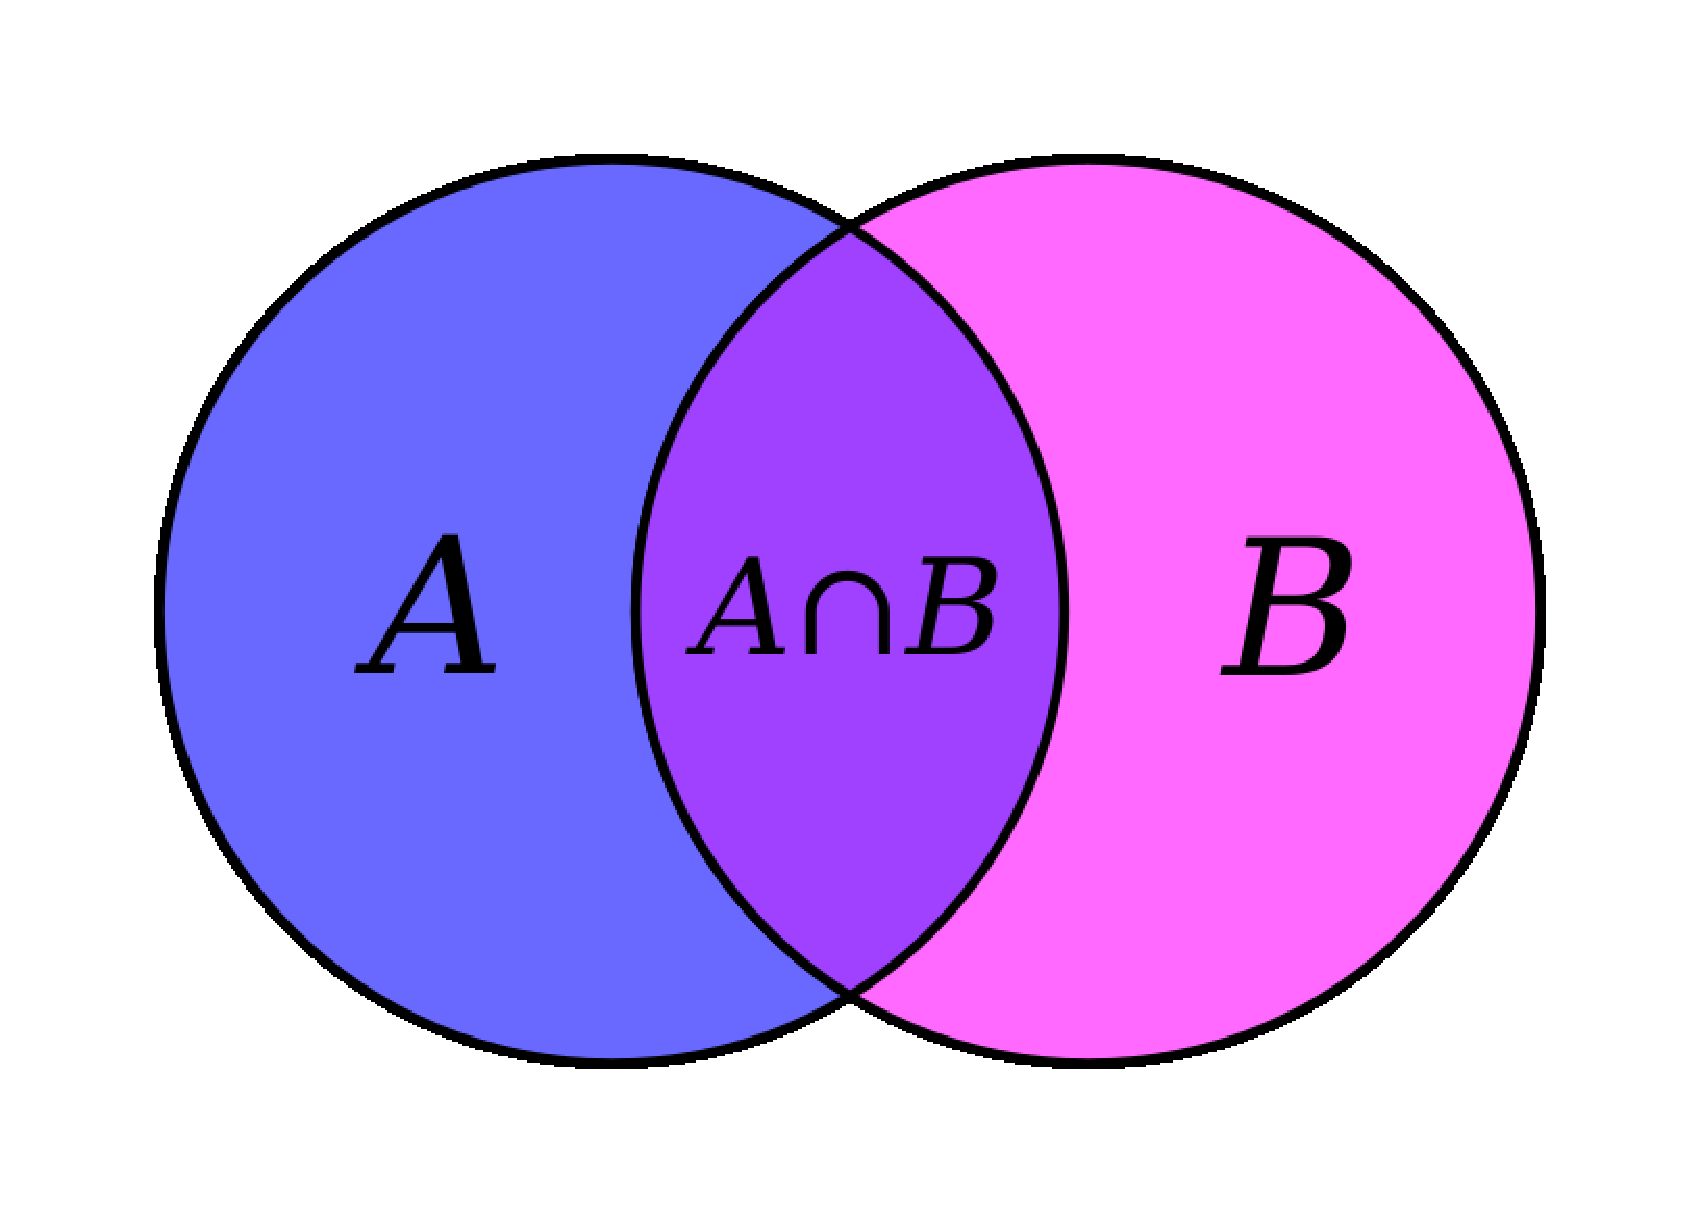
\includegraphics[scale=0.15]{venneuler.eps}\\
        \emph{Obrázek 1: Množiny A, B a jejich průnik}
    \end{center}

\section{Základní množinové operace}
    Mezi množinami můžeme provádět různé množinové operace. Mezi nejzákladnější patří sjednocení, průnik, rozdíl a doplněk.~\cite{MathWeb2022}
    \begin{itemize}
        \item \textbf{Sjednocení}: ${A \cup B = C}$
        \item \textbf{Průnik}: ${A \cap B = D}$
        \item \textbf{Rozdíl}: ${A \setminus B = E}$
    \end{itemize}
    
    \subsection*{Sazba matematických symbolů}
    Příkazy {\fontfamily{qcr}\selectfont \string\cup}, {\fontfamily{qcr}\selectfont \string\cap} a {\fontfamily{qcr}\selectfont \string\setminus} jsou časti balíčku {\fontfamily{qcr}\selectfont amssymb}~\cite{heinken}
    
    \vfill

    Pro pohodlnost tady~\cite{Mendel2022} je seznam často užívaných symbolů při práci s množinami.
\newpage
\bibliographystyle{czechiso.bst}
\bibliography{proj4.bib}
\end{document}